\documentclass[tikz, border=5pt]{standalone}
\usepackage{amsmath} % for \dfrac
\usepackage{pgfplots}
\usepgfplotslibrary{groupplots}

% \usetikzlibrary{decorations.pathreplacing,decorations.markings}
\usetikzlibrary{arrows.meta}


\pgfplotsset{every axis/.append style={
                    axis x line=middle,    % put the x axis in the middle
                    axis y line=middle,    % put the y axis in the middle
                    axis line style={<->,color=blue}, % arrows on the axis
                    xlabel={$x$},          % default put x on x-axis
                    ylabel={$y$},          % default put y on y-axis
            }}
\begin{document}
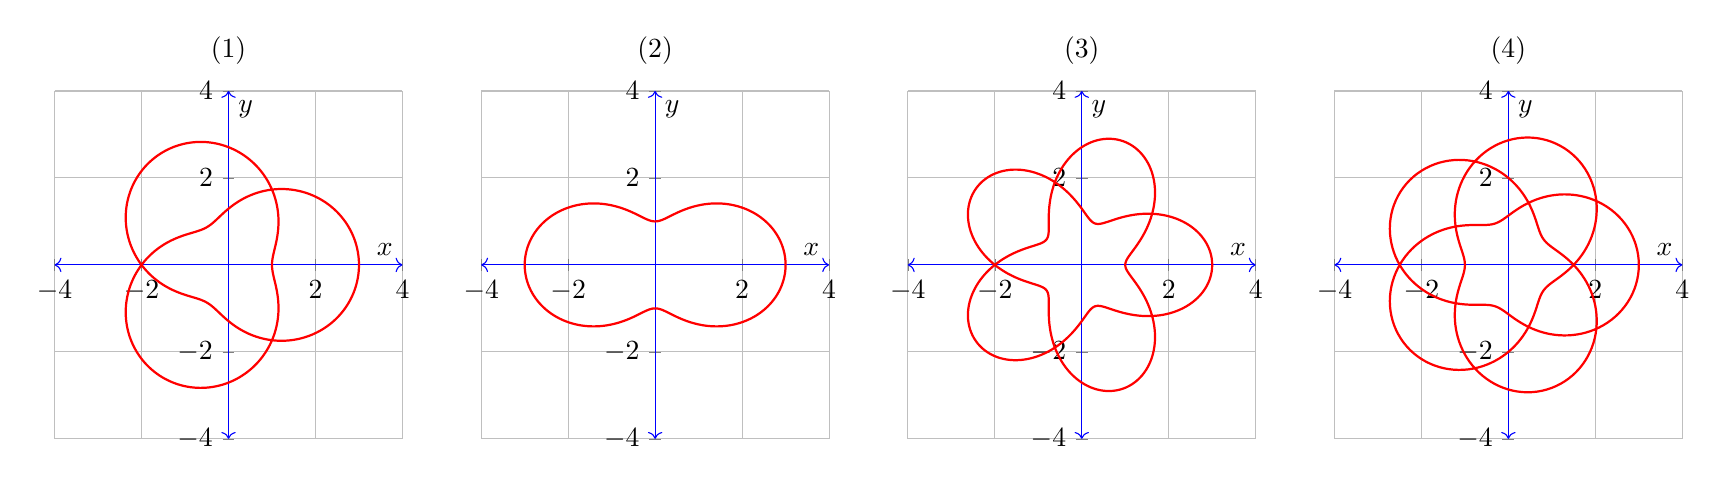
\begin{tikzpicture}
\begin{groupplot}[
    group style={group size={4 by 1}}, 
    height={6cm}, width={6cm},
    xmin=-4,xmax=4,
    ymin=-4,ymax=4,
    grid=both,
    ]
    \nextgroupplot[title={(1)}]
    \addplot [domain=-0:360, samples=500, thick, red]({(2+cos(3*x))*cos(2*x)},{(2+cos(3*x))*sin(2*x)}); 
    
    \nextgroupplot[title={(2)}]
    \addplot [domain=-0:360,samples=500, thick, red]({(2+cos(4*x))*cos(2*x)},{(2+cos(4*x))*sin(2*x)}); 
    
    \nextgroupplot[title={(3)}]
    \addplot [domain=-0:360,samples=500, thick, red]({(2+cos(5*x))*cos(2*x)},{(2+cos(5*x))*sin(2*x)}); 

    \nextgroupplot[title={(4)}]
    \addplot [domain=-0:360,samples=500, thick, red]({(2+cos(5*x))*cos(3*x)},{(2+cos(5*x))*sin(3*x)}); 

\end{groupplot}

\end{tikzpicture}
\end{document}
